\subsection{Organisation}

\begin{frame}{Organisation}

\begin{figure}
  \begin{center}
    \leavevmode
      \includegraphics[width = .75\textwidth]{organisation}
    \caption{Scrum Master und Product Owner}
  \end{center}
\end{figure}

\end{frame}

\pagebreak

\begin{frame}{Organisation}

	\pause
	\"Ubersicht:
	\pause
	\begin{itemize}
		\item Anforderungen, Ziele und Prozesse
		\pause
		\item Team-Aufteilung 
		\pause
		\item Aufgetretene Probleme und gefundene L\"osungen
		\pause
		\item Verwendete Tools
		\pause
		\item Vorstellung der Compiler Pipeline
	\end{itemize}

\end{frame}

\pagebreak

\begin{frame}{Organisation: Anforderungen, Ziele und Prozesse}

	\pause
	\begin{itemize}
		\item Bau eines Compilers f\"ur Rail in C++ zu Java Bytecode (selbstgew\"ahltes Target)
		\pause
		\item Rail ist eine zweidimensionale, esoterische Programmiersprache 
		\pause
		\item Der komplette Sprachumfang soll umgesetzt werden
		\pause
		\item Dieses \"ubergeordnete Ziel wurde unterteilt in 3 Meilensteine:
		\pause
		\begin{itemize}
			\item \textbf{\textcolor{fu-blue}{MS 1}}  Grundlegendes Parsen der Schienen, Strings und Konsolenausgabe
			\pause
			\item \textbf{\textcolor{fu-blue}{MS 2}}  Arithmetische Operationen, Verzweigungen (if-else) und Variablen
			\pause
			\item \textbf{\textcolor{fu-blue}{MS 3}}  Kompletter Sprachumfang: Funktionsaufrufe, Rekursion, Schleifen 
		\end{itemize}
	\end{itemize}

\end{frame}
	
\begin{frame}{Organisation: Anforderungen, Ziele und Prozesse}

	\pause
	\begin{itemize}
		\item Zus\"atzliche Anforderungen:
		\pause
		\begin{itemize}
			\item \textbf{\textcolor{fu-blue}{Cross-Kompatibilit\"at}} Erstellung eines austauschbaren Dateiformats f\"ur den AST
			\pause
			\item \textbf{\textcolor{fu-blue}{Cross-Testing}} Testen der Compiler der zwei Gruppen mit Ast-Dateien der jeweils anderen Gruppe
			\pause
			\item \textbf{\textcolor{fu-blue}{IDE}} Eine f\"ur Rail spezialisierte Entwicklungsumgebung soll umgesetzt werden
			\pause
		\end{itemize}
		\item Prozess ist Scrum-\"ahnlich:
		\pause
		\begin{itemize}
			\item Meilensteine (Sprints)
			\pause
			\item Stand-up Meetings
			\pause
			\item Retrospektiven (am Ende der Meilensteine)
			\pause
			\item Rollen wie Scrum Master und Product Owner
		\end{itemize}
	\end{itemize}

\end{frame}

\pagebreak


\begin{frame}{Verwendete Tools}

	\pause
	\begin{itemize}
		\item Teamspeak
		\pause
		\item Jabber
		\pause
		\item Mail 
		\pause
		\item Github als Codebase
		\pause
		\item Keine festgelegte Entwicklungsumgebung f\"ur C++
		\pause
		\item Jenkins und Gradle f\"ur Continuous Integration
		\pause
		\item Qt f\"ur die Entwicklung des Editors
		\pause
		\item Doxygen f\"ur automatisierte Dokumentationserzeugung
	\end{itemize}


\end{frame}


\begin{frame}{Organisation: Team-Aufteilung}

\begin{figure}
  \begin{center}
    \leavevmode
      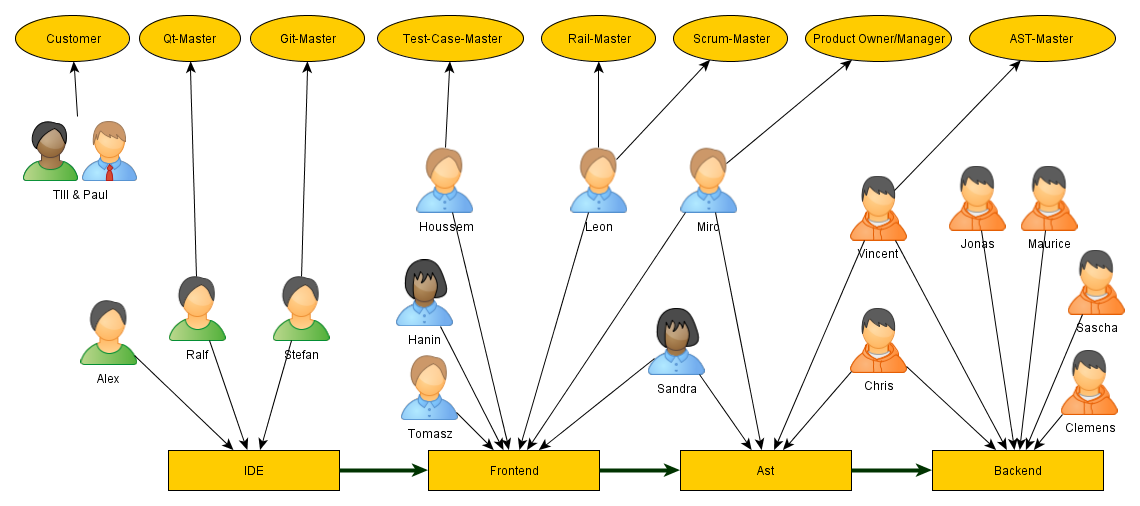
\includegraphics[width = \textwidth]{organigram}
    \caption{Organigramm}
  \end{center}
\end{figure}

\end{frame}

\pagebreak

\begin{frame}{Organisation: Aufgetretene Probleme und gefundene L\"osungen}
	
	\pause
	\begin{itemize}
		\item Probleme in MS 1:
		\pause
		\begin{itemize}
			\item Kommunikation (kein einheitliches Tool, seltene Treffen)
			\pause
			\item Unklare bzw. ungleiche Arbeitsaufteilung
			\pause
		\end{itemize}
		\item Verbessert durch:
		\pause
		\begin{itemize}
			\item Einf\"uhrung von Daily-Scrums $\rightarrow$ 3 Treffen pro Subteam w\"ochentlich (Voice-Chat)
			\pause
			\item Scrum-Master und Product Owner sind bei allen Treffen anwesend $\rightarrow$ besserer Gesamt\"uberblick
			\pause
			\item Nutzung der Github-Issues zur Verbesserung und Klarstellung der Aufgabenverteilung
			\pause
			\item Jabber f\"ur spontane Kommunikation
		\end{itemize}
	\end{itemize}
	
\end{frame}

\begin{frame}{Vorstellung der Compiler Pipeline}

\begin{figure}
  \begin{center}
    \leavevmode
      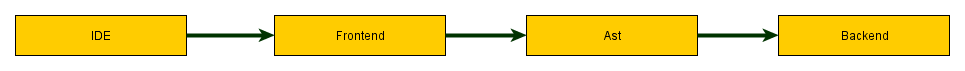
\includegraphics[width = \textwidth]{pipeline}
    \caption{Compiler Pipeline und Subteams}
  \end{center}
\end{figure}

\end{frame}
